\documentclass[conference]{IEEEtran}
\IEEEoverridecommandlockouts
% The preceding line is only needed to identify funding in the first footnote. If that is unneeded, please comment it out.
\usepackage{cite}
\usepackage{amsmath,amssymb,amsfonts}
\usepackage{algorithmic}
\usepackage{graphicx}
\usepackage{textcomp}
\usepackage{xcolor}
\usepackage{hyperref}
\def\BibTeX{{\rm B\kern-.05em{\sc i\kern-.025em b}\kern-.08em
    T\kern-.1667em\lower.7ex\hbox{E}\kern-.125emX}}
\begin{document}
\title{Monitoring the Results with Machine Learning Techniques for Real-time Healthcare}

\author {
    \IEEEauthorblockN{
    Ngo Bao Lam\IEEEauthorrefmark{1},
    Nguyen Do Truc Quynh\IEEEauthorrefmark{1},
    Tran Viet Tuan\IEEEauthorrefmark{1},
    Bui Long Toan\IEEEauthorrefmark{1},
    Nguyen Kim Thinh\IEEEauthorrefmark{1},\\
    Thi Thuy Hoai Nguyen\IEEEauthorrefmark{1},
    and Luong Vuong Nguyen\IEEEauthorrefmark{2}\thanks{Corressponding author: vuongnl3@fe.edu.vn}
    }
    
    \IEEEauthorblockA {
    \IEEEauthorrefmark{1}Department of Software Engineering, FPT University, Danang 550000, Vietnam\\
    \IEEEauthorrefmark{2}Department of Artificial Intelligence, FPT University, Danang 550000, Vietnam\\
    Email: vuongnl3@e.edu.vn
    }
}


\maketitle


\begin{abstract}
The explosion of medical data and the need for instant decisions in clinics are pushing the boundaries of how we use patient information. This study dives into how machine learning can be used to analyze mountains of patient records and turn them into actionable insights in real-time. Imagine doctors having a powerful tool that can predict things like how a disease might progress, whether a patient might need to come back to the hospital, or even how well a treatment might work. That's the potential of this research!

Our approach involved cleaning up and organizing all sorts of patient data, from demographics and medical history to test results and treatment plans. Then, we used powerful machine learning models, like those fancy deep learning algorithms you might hear about, to predict different health outcomes.

Here's the exciting part: we built a web platform that uses these techniques! This platform lets users input their data, track it over time, and even personalize it to their needs. An important feature is a built-in chatbot, so users can get feedback and answers to their questions.

The results are promising! This platform has the potential to be a game-changer for doctors by giving them real-time support when making decisions. Ultimately, this could lead to better care for patients and a more efficient healthcare system. This study is a stepping stone towards a future where artificial intelligence becomes a regular part of healthcare, allowing for more proactive and personalized care for everyone.
\end{abstract}

\begin{IEEEkeywords}
machine learning, monitoring, real-time healthcare

\end{IEEEkeywords}

\section{Introduction}

The healthcare field is overflowing with data these days. It's a double-edged sword - we have tons of information, but how do we use it to truly help patients? That's where this new research comes in. Machine learning is like a superpowered translator, taking mountains of medical records and turning them into clear messages doctors can use right away to make better decisions.

This study explored how machine learning can analyze patient data and predict things like how a disease might progress, whether a patient might need to come back to the hospital, or even how well a treatment might work. The researchers first cleaned up and organized all sorts of patient information, from basic details like age and address to their treatment history. Then, they used powerful machine learning models to predict these important health outcomes.

Here's the coolest part: they built a website that uses these techniques! Patients can enter their data, track it over time, and even personalize it to their specific needs. There's even a built-in chat feature, so users can get feedback and answers to their questions directly.

The results are exciting! This platform could be a game-changer for doctors by giving them real-time support when making decisions. Ultimately, it could lead to better care for patients and a more efficient healthcare system. This research is paving the way for a future where artificial intelligence works hand-in-hand with doctors to deliver proactive and personalized care for everyone.
    
    %Bổ sung các nghiên cứu về Chatbot và ứng dụng của nó vào lĩnh vực chăm sóc sức khỏe
    The integration of chatbots powered by artificial intelligence (AI), particularly machine learning (ML), into healthcare systems has gained significant momentum in technologically advanced countries. This trend reflects a growing interest in leveraging AI to enhance healthcare delivery.

    A seminal paper by Athota et al. (2020) \cite{athota2020chatbot} proposed a healthcare chatbot utilizing AI to deliver medical information, offer diagnostic support, and connect patients to healthcare professionals. This chatbot employs natural language processing (NLP) techniques to comprehend patient queries and generate appropriate responses. The study evaluated the chatbot's effectiveness through real-user testing and demonstrated its ability to provide accurate and useful medical information to patients.
    
    Building upon this research, Xu et al. (2021) \cite{xu2021chatbot} conducted a systematic review of chatbots utilizing AI and ML within healthcare and oncology applications. Their comprehensive search, spanning databases like PubMed, MEDLINE, and Scopus, targeted articles published between 2010 and August 2020. The review identified 55 relevant studies, highlighting the growing body of research in this field. These findings underscore the vast potential for chatbot applications within healthcare, paving the way for future advancements.

    %Liệt kê dạng itemize contribution của bài báo
    In recap, the contribution of this study can be summarized as follows:
    \begin{itemize}
          \item \textbf{Unlocking Patient Insights:} This research unveils a powerful machine learning toolkit that analyzes a wide range of patient data, using techniques like support vector machines and deep learning. This allows us to uncover hidden patterns and predict future health trends.
          \item \textbf{Proactive Healthcare:} Imagine being able to anticipate potential health issues before they arise. Our framework empowers doctors to intervene early, potentially preventing complications and improving overall patient outcomes.
          \item \textbf{Your Health By Your Way:} We've developed a user-friendly web platform that puts you in control of your health journey. It allows you to easily collect and analyze your data, track your progress, and receive personalized health insights.
          \item \textbf{Chatting Your Way to Better Health:} We've integrated a chatbot into the platform, making it easier than ever to get answers to your questions and access important information. This fosters a more interactive healthcare experience and empowers you to take an active role in managing your health.
        \end{itemize}
    
    %Thay Vuong
    The remainder of this manuscript is structured as follows. Section~\ref{method} explores techniques for data extraction, question answering, and entity recognition in healthcare documents. This includes an OCR pipeline for digitizing scanned documents, a chatbot system for answering user queries, and the application of YOLO V8 for improved OCR accuracy. Additionally, fine-tuning methods are employed to optimize question-answering performance. In Section~\ref{experimental}, we discussed and evaluated these methods with a curated dataset and metrics. Finally, we summarize our findings and show the directions for future work in Section~\ref{conclusions}.

\section{Literature Review}
\label{literature}
    Numerous investigations covering the healthcare domain have jointly underscored the revolutionary capacity of machine learning (ML) to markedly improve diverse facets of medical practice. One of the most significant developments made possible by machine learning (ML) is its unmatched capacity to identify illnesses with a degree of precision that was previously unachievable using traditional methods. These studies have repeatedly demonstrated the superiority of ML algorithms in the analysis of intricate datasets, the discovery of subtle patterns, and the extraction of significant insights that aid in the prompt and more accurate diagnosis of diseases.

    %Cite paper vào
   Additionally, scholars like Rajkomar et al. (2018) \cite{rajkomar2018scalable} have conducted thorough analyses contrasting machine learning algorithms' predictive efficacy with traditional statistical techniques. Their findings demonstrate the effectiveness of machine learning techniques by demonstrating their ability to predict patient outcomes with unprecedented precision, beating more conventional methods. By leveraging complex computer algorithms and big datasets, machine learning (ML) models enhance prognosis accuracy and give medical professionals invaluable prediction insights that can direct customized treatment regimens and improve patient outcomes.

    %Cite paper vào
 Furthermore, there is great potential for transforming healthcare delivery through the integration of ML-driven diagnostic and prognostic tools into clinical practice. These developments set the stage for a time when data-driven insights will increasingly influence medical decisions, resulting in better patient outcomes, more effective use of resources, and tailored treatment regimens. To fully realize the promise of precision medicine and usher in a new era of revolutionary healthcare innovation, ML technologies must be further explored and adopted in the healthcare industry. The use of machine learning models for predictive analytics in healthcare settings is examined in the paragraph that follows, which turns the focus to the applications of these developments. A lot of research has been done on the effectiveness of machine learning (ML) models in clinical settings, with a particular emphasis on models like support vector machines and neural networks. Several studies, such as the thorough examination conducted by Beam and Kohane (2018) \cite{yu2018artificial}, have carefully assessed these models using a variety of clinical datasets. These studies go far into comprehending the adaptability and performance metrics of machine learning models to various and intricate healthcare contexts. Through a methodical investigation of their application in clinical decision-making processes in real-time, scientists have clarified the complex properties of machine learning models, revealing their potential to completely transform medicine. These extensive analyses highlight how important it is to include sophisticated predictive analytics in healthcare processes, which will eventually open the door for patient care plans that are better informed and more successful. However, data quality is a critical component that must be met to fully utilize these ML models. These algorithms use data as their starting point for learning and prediction.  As a result, it becomes crucial to guarantee the accuracy, completeness, and relevance of healthcare data.

    %Cite paper vào
    There is broad recognition in the literature for the crucial roles that feature selection and data quality play in machine learning. Luo et al. (2016) \cite{luo2016review} explore preprocessing techniques for healthcare data in their groundbreaking work, providing significant insights on guaranteeing the resilience and reflectiveness of inputs to machine learning models. Their thorough analysis covers a variety of approaches to improve data integrity, highlighting the necessity of thorough preparation methods that take into consideration the complexities of clinical occurrences.

    %Cite paper vào
    Luo et al. (2016) \cite{luo2016review} emphasize the value of feature engineering and emphasize the significance of data quality in boosting the effectiveness of machine learning models by carefully examining various preprocessing techniques. They clarify the complex relationship between feature selection, data preprocessing, and the overall effectiveness of ML algorithms in healthcare situations by their thorough analysis.

    %Cite paper vào
    Additionally, their investigation of the best techniques for preparing healthcare data is a vital contribution to the field's advancement, offering practitioners and researchers priceless advice on how to maximize the relevance and integrity of data inputs. Researchers can guarantee that machine learning models receive precise, clinically relevant inputs by following these techniques, which will enable more impactful and reliable insights into patient care and treatment outcomes. Beyond data quality, machine learning is successfully applied in the healthcare industry. Its deployment's ethical implications are just as significant. The use of machine learning (ML) in the healthcare industry presents significant challenges and ethical considerations that are receiving more and more attention from the academic and professional communities. Although there is no denying that machine learning (ML) has the potential to completely transform healthcare, there are several moral conundrums and issues that must be taken into account before using ML. Char et al. (2018) \cite{char2018implementing} delve into these ethical implications, offering a thought-provoking analysis emphasizing the delicate balance between technological innovation and safeguarding fundamental patient rights, including data privacy.

    %Cite paper vào
Char et al. (2018) \cite{char2018implementing} carefully analyze the moral dilemmas associated with incorporating ML technology into healthcare systems in their groundbreaking study. They draw attention to the moral conundrums brought on by the massive processing and analysis of private patient data, raising worries about possible violations of people's right to privacy. The authors also stress the significance of guaranteeing interpretability and openness in machine learning algorithms, since opaque models have the potential to worsen biases and inequality already present in healthcare systems.

    %Cite paper vào
Furthermore, Char et al. (2018) \cite{char2018implementing} support a comprehensive framework that prioritizes patient autonomy, beneficence, and justice to support a holistic approach to ethical decision-making. Their perceptive study highlights the moral obligations that come with creating, implementing, and overseeing machine learning (ML) technologies in the healthcare industry. It also exhorts relevant parties to take proactive measures to confront these issues to preserve moral principles and advance fair access to high-quality healthcare. While morality plays a major role, user-friendly platforms are also essential to converting machine learning's promise into real advantages for patients.

    %Cite paper vào
   The seamless integration of machine learning (ML) models into user-friendly platforms has huge promise for enhancing patient care and optimizing healthcare operations, which has led to a growing focus on integration with healthcare platforms within the healthcare sector. In-depth research in this field has been done by Topol (2019) \cite{topol2019deep}, who looks at how healthcare platforms can be strategically built to collect data and enable meaningful user interactions. These platforms can leverage chatbots and other interactive features to improve user engagement and streamline data management procedures.

    %Cite paper vào
    Topol's (2019) \cite{topol2019deep} study highlights how ML-powered platforms can revolutionize the provision of healthcare. Healthcare practitioners can obtain real-time insights and predictive analytics through the integration of advanced machine learning algorithms, which empowers them to make well-informed decisions and more effectively customize treatment programs. Furthermore, these platforms expedite care coordination and advance patient-centered approaches to healthcare by encouraging increased collaboration and communication among stakeholders.

    In addition to improving patient care, integrating ML into healthcare platforms necessitates robust data security measures. Topol (2019) \cite{topol2019deep} highlights the importance of implementing encryption protocols and data protection measures to safeguard sensitive patient information and mitigate cybersecurity risks.

    All things considered, the incorporation of machine learning into healthcare systems is a noteworthy development in the area, providing fresh opportunities to improve patient outcomes and healthcare delivery. Topol's (2019) \cite{topol2019deep} research plays a crucial role in this dynamic environment by opening doors for creative approaches that use technology to raise the standard, accessibility, and effectiveness of healthcare services. But to fully realize the potential of these platforms, sophisticated machine-learning models and efficient user-interaction techniques are needed. Human-Computer Interaction (HCI) is relevant in this situation.\\
    
    Advances in deep learning and natural language processing (NLP) have enabled human-computer interaction (HCI) to go beyond basic mouse clicks and slider movements. A growing field in HCI is chatbots, or machine agents using natural language interfaces. Users and data or service providers can naturally communicate using these interfaces. Chatbots, or machine agents that act as natural language user interfaces for data and service providers, are becoming more and more popular. "Productivity" is the most often mentioned motivating factor; chatbots assist users in obtaining information or support quickly and effectively. In addition, users of chatbots mentioned being motivated by social and relational aspects, amusement, and curiosity about what they perceive to be a new phenomenon. \cite{folstad2017chatbots}. 
    
  The prevalence of automated chatbots in customer assistance across several businesses is undeniable. Artificial intelligence (AI) virtual assistants, like Apple's Siri, Amazon's Alexa, and Microsoft's Cortana, are progressively taking the place of human agents in repetitive conversational tasks. This invention is motivated by the need to streamline customer assistance procedures and lessen the workload for human agents. As a result, more companies are actively integrating chatbots into their customer support platforms. Vietnamese chatbots are not well-documented, although they are already widely used in numerous industries. The bulk of these projects are still closed-source, and the advancement of these efforts is not well documented in academic journals.
    
While Vietnamese chatbots are mostly closed-source projects, research on English chatbot systems has blossomed.  There are very few research articles accessible that discuss the creation of these chatbots; most of the work is still unrecorded in academic journals. There are just two published studies on this topic, making the literature on it somewhat thin. In the real estate industry, the first was creating a chatbot for lead engagement \cite{quan2018lead}. A different study focuses on a chatbot tutor for high school pupils that provides them with solutions suggestions instead of giving them straight answers \cite{nguyen2020design}. In order to close this research gap and build reliable chatbots in Vietnamese, developers need to take care of a number of important technological issues, especially with regard to Natural Language Understanding (NLU).
    
   An essential stage in Natural Language Understanding (NLU) is intent categorization, which helps chatbots determine the rationale behind human statements and direct the flow of the discussion. For unstructured data, such as chat discussions, many categorization techniques work well. These include deep learning designs like Convolutional Neural Networks (CNN) and Recurrent Neural Networks (RNN), together with their specialized variations, and standard machine learning models like Support Vector Machines (SVM) and Conditional Random Fields (CRF).
    
    Previous studies on the classification of Vietnamese intent show the potential of many methods. In one study, the combination of CRF with Long Short-Term Memory (LSTM), a kind of RNN, produced remarkable results for general-domain intent classification. \cite{luong2017intent}. Another study successfully classified user intent using a CNN with a Softmax output layer \cite{ngo2017identification}. Similarly, a real-estate-specific study utilized a combination of CNN and Bidirectional Gated Recurrent Unit (Bi-GRU), another RNN variant, followed by CRF \cite{quan2018lead}. Recent work combining Bi-LSTM with CNN and CRF also garnered promising results \cite{tran2020understanding}.
    
   Although deep learning has taken the lead in Vietnamese intent classification and context management, no discernible performance difference was discovered in a 2017 study that compared the performance of a traditional CRF model with a contemporary Bi-LSTM-CRF architecture on a dataset of text messages. \cite{ngo2017identification}.Traditional methodologies still have value, even though the gap between deep learning and current state-of-the-art technologies has expanded. Their usefulness as baselines is especially important in situations where there is a dearth of training data, like in intent classification tasks.

\section{Methodology}
\label{method}
    In the realm of scientific inquiry, methodology serves as the compass that guides our research journey, ensuring that we navigate the path of knowledge with rigor and precision. It is the backbone of our study, providing a transparent and replicable framework for our investigative endeavors.

    In this section, we meticulously unveil the methodology that underpins our research, outlining the steps we meticulously followed to unravel the complexities of our research problem. We will delve into the data acquisition and preparation processes, the analytical techniques employed, and the statistical methods utilized to extract meaningful insights from the vast sea of information.

    Prepare to embark on a journey of methodological transparency as we unveil the intricate details of our research approach.
    \subsection{OCR - Data Extraction Pipeline}
    Our system inputs an uploaded medical document image (e.g., prescription, exam report). The output of the system is the extracted health data from the document. The system first performs image preprocessing on the uploaded image, which may involve format validation, noise reduction, skew correction, and potentially binarization. Next, an Optical Character Recognition (OCR) engine extracts the text from the preprocessed image. The extracted text then undergoes postprocessing, including layout analysis (optional) and data-cleaning techniques like spell-checking and dictionary matching. Finally, the extracted health data (patient details, diagnosis, medication) is mapped to the corresponding fields in the health monitoring system's form for automatic population.
    
    \begin{figure}[htbp]
        \centerline{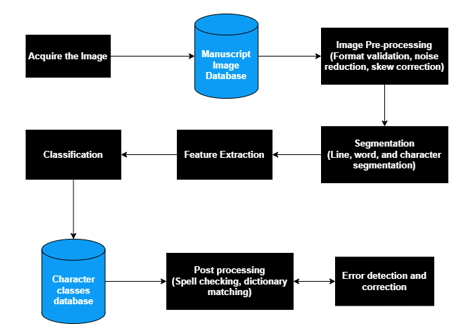
\includegraphics[scale=0.6]{Figures/OCR pipeline.PNG}}
        \caption{OCR - Data Extraction Pipeline.}
    \label{Fig. 1}
    \end{figure}

    The input of our system is a user query, and the system's output is a response to the query, both in the context of health information. The user query, which is natural language text, transforms features through a Natural Language Processing (NLP) process. These extracted features are then used to classify the intent of the user's question using machine learning models trained on a dataset of labeled conversation examples. Finally, the original user query and the results of the machine learning models (classified intent) are fed into a retrieval-based answering component to retrieve the most relevant response.
    
    \begin{figure}[htbp]
        \centerline{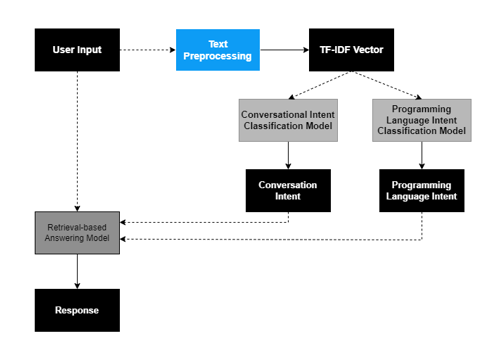
\includegraphics[scale=0.8]{Figures/Chatbot PipeLine.PNG}}
        \caption{Chatbot - Question Answering Pipeline.}
    \label{Fig. 2}
    \end{figure}

    \subsection{YOLO V8 for OCR in Healthcare}
    %Cite paper gốc của YOLO vào
    The YOLO (You Only Look Once) V8 model marks the latest evolution in the YOLO \cite{jiang2022review} series, renowned for its high-speed and accurate real-time object detection capabilities. This version introduces significant enhancements, including a more efficient backbone architecture, improved anchor-free detection heads, and sophisticated training methodologies. YOLO V8 typically operates with input resolutions ranging from 320x320 to 640x640 pixels, employs a confidence threshold to ascertain object detection accuracy, and utilizes non-maximal suppression (NMS) to refine the bounding boxes of detected objects. Its architecture consists of a feature extraction backbone, such as CSPDarknet53, a neck component like PANET for aggregating features, and head layers dedicated to object classification and localization.
    
    In healthcare, YOLO V8 can significantly streamline the OCR (Optical Character Recognition) process, particularly for digitizing medical examination results and prescriptions. By leveraging its object detection prowess, YOLO V8 can precisely identify and localize text regions within various medical documents. This capability is crucial for dealing with complex layouts and diverse font styles in handwritten and printed medical forms. Once detected, these text regions can be processed by OCR engines to extract pertinent information, such as medication names, dosages, and examination outcomes, which are then automatically populated into digital health records. This integration enhances data entry accuracy and efficiency and ensures that medical records are comprehensive and up-to-date, facilitating better personalized health recommendations via AI-powered chatbots.

    \subsection{Preprocessing and Feature Extracting using Fine-Tuning Method}
        \subsubsection{Medical Image Scanning}
        Medical imaging plays a crucial role in diagnosing and monitoring various medical conditions. However, the complex nature of these images makes extracting meaningful features for analysis challenging. Here, we propose a pipeline leveraging fine-tuning to overcome this hurdle.
        
        \begin{itemize}
          \item \textbf{Preprocessing:} This stage prepares the images for feature extraction and involves several steps:
            \begin{itemize}
                \item \textbf{Image Normalization:} Variations in intensity and contrast due to factors like patient positioning are addressed through normalization techniques, ensuring consistency for feature extraction.
                \item \textbf{Image Segmentation:} Isolating the region of interest (ROI) containing the abnormality from the background is crucial. Techniques like thresholding and edge detection help achieve this.
            \end{itemize}
          \item \textbf{Fine-Tuning with YOLOv8:} Once preprocessed, feature extraction is performed. We propose using a fine-tuned YOLOv8 model as an effective method. YOLOv8, a state-of-the-art object detection algorithm, excels in various computer vision tasks. We can train it to recognize and localize specific medical abnormalities with high accuracy by fine-tuning it on a medical image dataset.
        \end{itemize}
        Fine-tuning involves adjusting the YOLOv8 model's parameters to optimize its performance for medical image analysis. This includes defining object classes (e.g., tumor, lesion) and training the model to detect and localize them. The resulting fine-tuned model can then extract relevant features from new medical images, aiding diagnosis and treatment planning.

    \subsubsection{Vietnammese Medical Chatbot}
    Natural Language Processing (NLP) is pivotal in enabling effective medical chatbots. However, medical text data poses unique challenges due to specialized terminology and complex medical concepts. Preprocessing and feature extraction are crucial steps in NLP pipelines to prepare raw text data for machine learning models. Preprocessing involves cleaning and transforming the text to remove noise and inconsistencies, while feature extraction aims to identify and represent the most relevant information from the text.
    
    Preprocessing and feature extraction offer several benefits in the context of medical chatbots:
        \begin{itemize}
            \item \textbf{Improved Data Quality:} Preprocessing helps eliminate irrelevant information, such as punctuation, special characters, and HTML tags, ensuring the chatbot focuses on meaningful content.
            \item \textbf{Enhanced Feature Representation:} Feature extraction transforms raw text into a structured format that machine learning models can effectively process. This leads to a better understanding of the text and improved model performance.
            \item \textbf{Reduced Computational Complexity:} By extracting the most relevant features, feature extraction reduces the dimensionality of the data, making it easier for machine learning models to train and run efficiently.
        \end{itemize}

    Effective word embedding, a crucial step for Vietnamese language models, hinges on accurate word segmentation \cite{cong2016state}.
    \begin{figure}[!htbp]
        \centerline{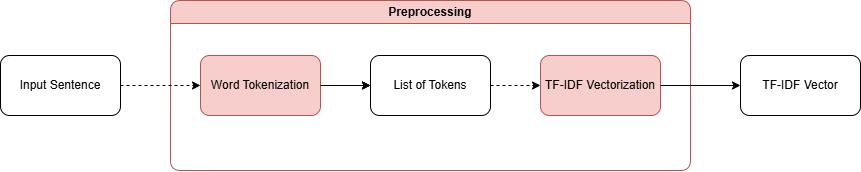
\includegraphics[width=0.5\textwidth]{Figures/preprocessing.png}}
        \caption{Preprocessing and Feature Extracting.}
    \label{Fig. 3}
    \end{figure}

    This is particularly important because Vietnamese text lacks explicit word boundaries, unlike languages with spaces between words. Word segmentation is critical in preprocessing Vietnamese text, as spaces do not always separate words. This becomes even more challenging in the medical domain due to multi-syllable medical terms and specialized jargon. To effectively handle these complexities, we implemented a three-pronged approach:
    
    \begin{itemize}
        \item \textbf{Medical Term Dictionary Integration:} A comprehensive medical term dictionary was integrated into the word segmentation process. This dictionary encompasses various medical terms, including common diseases, symptoms, medications, and anatomical structures.
        \item \textbf{Context-Aware Segmentation:} Context-aware segmentation techniques were employed that consider the surrounding words and phrases to identify medical term boundaries accurately. This helped distinguish between multi-syllable words and potential misspellings.
        \item \textbf{Domain-Specific Rule-Based Segmentation:} Domain-specific rules tailored to the medical domain were implemented. These rules handled common patterns in medical terminology, such as the presence of hyphens or prefixes.
    \end{itemize}

    Afterword segmentation, different techniques can be employed to represent words numerically, known as word embedding. These techniques include Bag-of-Words, TF-IDF, word2vec, doc2vec, and GloVe, each with its advantages and limitations. Deep learning-based embedding methods excel at capturing semantic relationships between words, but they often necessitate large datasets for training.

    Given the potential limitations in dataset size, we opted for Term Frequency-Inverse Document Frequency (TF-IDF) for vectorizing input utterances for our text classification models. TF-IDF considers both a word's frequency within a document (term frequency) and its rarity across the entire dataset (inverse document frequency), creating a robust representation of words. To further enhance information retrieval within the medical domain, we implemented a modified scheme that assigns higher weights to medical terms and calculates IDF values specific to different disease categories:
    \begin{itemize}
        \item \textbf{Medical Term Weighting:} Higher weights were assigned to medical terms within the TF-IDF calculations. This ensured that medically relevant terms were given greater prominence when retrieving information.
        \item \textbf{Disease-Specific IDF Calculation:} IDF values were calculated separately for different disease categories. This accounted for the varying distribution of medical terms across different disease domains.
    \end{itemize}

    A comprehensive medical corpus of medical articles, patient records, and clinical guidelines was constructed to support the NLP techniques. This corpus was the foundation for calculating TF-IDF weights and provided a rich source of medical text data for training and evaluation. The product of these two values, Term Frequency (TF) and Inverse Document Frequency (IDF), determines the TF-IDF score for a word within a document. This score indicates the relative importance of that word within that specific document. Higher TF-IDF scores signify greater relevance. Formally, the TF-IDF score (TF-IDF(t, d)) for a word t in document d within a document collection D can be expressed mathematically as:

    \begin{equation}
    \text{tf-idf}(t, d, D) = \text{tf}(t, d) \cdot \text{idf}(t, D)
    \end{equation}
    where: \\
    
    \begin{equation}
    \text{tf}(t, d) = \log(1 + \text{freq}(t, d))
    \end{equation}
    
    \begin{equation}
    \text{idf}(t, D) = \log \left( \frac{N}{\text{count}(d \in D : t \in d)} \right)
    \end{equation}

    \subsection{Intent Classification}
    Due to the potential limitations of our dataset size, we opted for a Support Vector Machine (SVM) for intent classification in our experiments. SVMs excel at binary classification by constructing a hyperplane that maximizes the margin between the training examples of two classes. Examples closest to this hyperplane are termed support vectors. During inference, unseen utterances are projected onto the same space and classified based on their position relative to the hyperplane.
    
    SVMs can be adapted to multiclass classification tasks using strategies like "one-vs-the-rest." This approach, often preferred in practice due to its linear scaling of hyperplanes with the number of classes, was employed in our experiments.
    
    Our chatbot aims to identify two main intent types within user utterances: conversational and programming language-related. Conversational intents encompass eleven categories: agreement, disagreement, credit information requests, greetings, requests for help, reference inquiries, tip requests, definition inquiries, comparisons, application inquiries, and out-of-context utterances. Programming language intents fall under three categories: general, C++, and Python. We trained separate "one-vs-the-rest" SVMs for each intent type to extract these intents.

    \subsection{Retrieval-based Answering}
    Our system utilizes an inference engine to determine the most suitable response based on rules and a knowledge base. Using machine learning models, this engine first identifies the user's intent from the current utterance. However, a "low confidence" intent is assigned if the model's prediction is uncertain (below a predefined threshold).
    
    \begin{figure}[htbp]
        \centerline{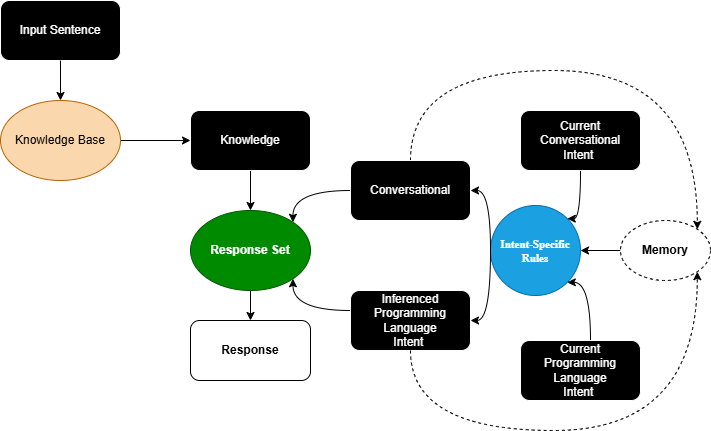
\includegraphics[scale=0.35]{Figures/retrieval.png}}
        \caption{Retrieval-based answering.}
    \label{Fig. 4}
    \end{figure}
    
    Intent-Specific Rules:
    \begin{itemize}
        \item \textbf{Programming Language Intent \(\mathbf{I_p}\):} Given a set of possible programming language tags (\(\mathbb{P} = \{\text{general, cpp, python}\}\)), the rules operate as follows:
            \begin{itemize}
                \item If the previous utterance's intent (\(\mathbf{I_{pt-1}}\)) differs from the current predicted intent (\(\mathbf{I_{pt}'}\)) and both belong to the set \(\mathbb{P}\), the final intent (\(\mathbf{I_{pt}}\)) is set to the current predicted intent.
                \item If the previous intent is a set containing any tag from \(\mathbb{P}\) and the current predicted intent is "low confidence," the final intent remains the previous intent.
                \item If both the previous and current predicted intents are "low confidence," the final intent is set to "general."
                \end{itemize}
        \item \textbf{Conversational Intent \(\mathbf{I_g}\): } Given a set of possible conversational intent tags (\(\mathbb{G} = \{
            \text{agree}, \linebreak 
            \text{ask\_application, ask\_comparison, ask\_credit\_info}, \linebreak
            \text{ask\_definition, ask\_references, ask\_tips, disagree}, \linebreak
            \text{greeting, need\_help, out-of-context, low\_conf}
            \}\), the rules operate as follows:
                \begin{itemize}
                    \item If the previous utterance's intent (\(\mathbf{I_{gt-1}}\)) differs from the current predicted intent (\(\mathbf{I_{gt}'}\)) and both belong to the set \(\mathbb{G}\), the final intent (\(\mathbf{I_{gt}}\)) is set to the current predicted intent.
                    \item If the previous intent is a set containing any tag from \(\mathbb{G}\) and the current predicted intent is limited to "agree" or "disagree," the final intent is set to "out-of-context."
                    \item If both the previous and current predicted intents are "low confidence," the final intent is set to "out-of-context."
                \end{itemize}
    \end{itemize}

    Knowledge Base:
    \begin{itemize}
        \item \(E\): Programming entity extracted from the user's utterance using regular expressions.
        \item \(\mathbf{I_p}\): Programming language tag.
        \item \(\mathbf{I_g}\): Query type tag (ask\_application, ask\_comparison, or ask\_definition).
        \item \(K\): Corresponding knowledge about the entity.
    \end{itemize}
    Response Set:
    The response set holds retrievable response patterns. Each pattern is a tuple in the format \((\{I_i \in I\}, R)\), where:
    
    \begin{itemize}
        \item \(I\): Set of extracted intents from the user's utterance.
        \item \(R\): List of possible response templates.
    \end{itemize}
    The system selects a random template from \(R\) to construct the final answer. By combining these components, the chatbot can generate appropriate responses and guide the conversation towards pre-defined topics related to programming knowledge.

\section{Experimental Result}
\label{experimental}
    In the realm of scientific inquiry, the Experimental Results section serves as the grand unveiling, where the curtains are drawn back to reveal the fruits of our research labor. It is the culmination of our meticulous efforts, showcasing the evidence that validates our hypotheses and illuminates the path toward knowledge advancement.
    
    Prepare to be captivated by the tapestry of results that unfolds before you, as we unveil the insights that our research has unearthed. Join us as we delve into the realm of experimental outcomes, where the power of data and analysis converge to reveal the hidden truths that underpin our research problem.
    \subsection{Overview Electronic Health Records (EHRs) Platform}
    Our study's main data source is Electronic Health Records (EHRs), which include treatment plans, clinical data, demographics, medical histories, and clinical notes. The data is thoroughly prepared to guarantee its quality and usefulness for analysis. The article emphasizes the importance of evaluation metrics in ensuring medical information accuracy and improving user experience in chatbot and OCR systems. The goals are to enhance the application's quality and successfully satisfy user needs.
    
    \subsection{Dataset}
    Our research primarily utilizes Electronic Health Records (EHR) as the foundational data source. EHRs provide a detailed and comprehensive record of patients' medical histories, encompassing demographics, clinical data, clinical notes, and treatment plans. Additional data sources such as wearable devices, social determinants of health, and public health databases may be integrated depending on specific research objectives. Following data acquisition, a rigorous preprocessing phase ensures data quality and analytical suitability. This phase addresses missing values, standardizes data formats, and may involve feature engineering to create new features pertinent to the research objectives.

    \begin{itemize}
        \item Our investigation leverages Electronic Health Records (EHR) as the primary data source, offering a comprehensive record of patients' medical history. This data encompasses demographics, medical history, clinical data, clinical notes, and treatment plans. Additionally, depending on the specific research objectives, we may incorporate data from wearable devices, social determinants of health, and public health databases. Following data acquisition, a meticulous preprocessing phase ensures data quality and suitability for analysis. This phase addresses missing values, standardizes data formats, and potentially involves feature engineering to create new features relevant to the research question.
    
        \item For supervised learning models intended to predict specific health outcomes, data annotation is a critical step. This process involves meticulously assigning labels (categories or values) to 18 different data points, thus transforming raw data into a format that machine learning models can interpret. Physician expertise is often leveraged for data annotation, where clinicians apply their clinical knowledge to assign diagnoses, treatment responses, or anticipated outcomes to data points. Alternatively, event-based labeling is employed to meticulously label specific health events of interest within the data. Table \ref{tab:classes} lists the specific labels we consider.
    
        \begin{table}[htbp]
        \centering
        \addtolength{\tabcolsep}{4pt}
        \def\arraystretch{1.5}
        \caption{\textnormal{Overview of annotated classes}}
        \label{tab:classes}
        \begin{tabular}{l l p{3cm}}
            \hline
            \textbf{Category} & \textbf{Class} & \textbf{Description} \\
            \hline
            \textbf{Demographics} & Patient Info & Basic information such as age, gender, etc. \\
            \hline
            \textbf{Medical History} & Diagnosis & Conditions and illnesses diagnosed \\
            & Treatment & Administered treatments \\
            & Prescriptions & Medications prescribed \\
            & Clinical Notes & Notes from clinicians on patient care \\
            \hline
            \textbf{Vital Signs} & Height & Patient's height \\
            & Weight & Patient's weight \\
            & Blood Pressure & Blood pressure readings \\
            & Heart Rate & Heart rate \\
            & Temperature & Body temperature \\
            & BMI Index & Body Mass Index \\
            \hline
            \textbf{Imaging} & Ultrasound Scans & Ultrasound images \\
            \hline
            \textbf{Financial} & Total Cost & Total cost of treatments and prescriptions \\
            \hline
            \textbf{Temporal Data} & Visit Date/Time & Date and time of visits \\
            \hline
            \textbf{Clinical Advice} & Recommendations & Medical advice given \\
            \hline
            \textbf{Administrative} & Location & Location of medical services \\
            & Department & Medical department or specialization \\
            \hline
            \textbf{Metadata} & Timestamps & Record creation and update times \\
            \hline            
            \end{tabular}        
        \end{table}
    
        \item Maintaining patient privacy and data security is paramount in healthcare research. The collected data will be housed in a secure environment to uphold these ethical and legal imperatives. This environment will leverage a HIPAA-compliant cloud storage solution, ensuring adherence to the most stringent healthcare data privacy regulations. Additionally, we will implement robust anonymization techniques to further shield patient identities. These techniques might involve removing direct identifiers like names and social security numbers while preserving the value of the data for research purposes. The specifics of data anonymization will be further elaborated upon in the Methodology section.        
    \end{itemize}
    
    \subsection{Evaluation Metrics}
    Users may now obtain medication information, make appointments, and communicate with doctors online using chatbots and optical character recognition (OCR) technology integrated into web apps for medical prescription scanning. Chatbot and OCR system performance evaluation is essential to guarantee the accuracy of medical information and improve user experience. This document contributes to improving the application's quality, and better meeting user demands by thoroughly examining performance assessment metrics for each component.

        \subsubsection{Chatbot}        
        Task Completion Rate (TCR): This measure represents the proportion of users who effectively complete their intended tasks with the chatbot's help. A high TCR indicates that the chatbot was successful in helping users reach their goals.
        
        Question Answering Accuracy: This indicator shows the percentage of queries sent to the chatbot that result in precise answers. It displays the chatbot's degree of comprehension and efficient information processing.
        
        %Cite bài báo gốc về các chỉ số đánh giá này vào
        F1-Score: This metric incorporates precision and recall beyond traditional accuracy measures. Precision refers to the proportion of correct responses among the chatbot's responses. Conversely, Recall focuses on the proportion of correctly answered questions out of all relevant questions. A high F1-Score indicates a well-balanced performance in terms of both precision and recall. It is calculated using the following formula \cite{goutte2005probabilistic}:
        
        \begin{equation}
            F1\text{-Score} = 2 \cdot \frac{\text{Precision} \cdot \text{Recall}}{\text{Precision} + \text{Recall}}
        \end{equation}
        
        Precision: This metric focuses on the positive class, which might represent a correct diagnosis suggestion or medication information retrieval in the context of a medical chatbot. It is calculated using the following formula \cite{goutte2005probabilistic}:
        
        \begin{equation}
        \text{Precision} = \frac{\text{True Positives}}{\text{True Positives} + \text{False Positives}}
        \end{equation}
        
        Recall: This metric emphasizes the model's sensitivity towards the positive class. In a medical chatbot scenario, it measures the proportion of actual positive cases that the chatbot correctly identified. It is calculated using the following formula \cite{goutte2005probabilistic}:
        
        \begin{equation}
        \text{Recall} = \frac{\text{True Positives}}{\text{True Positives} + \text{False Negatives}}
        \end{equation}

        \subsubsection{Optical Character Recognition (OCR)}
        
        Processing Time: Processing time measures the amount of time the OCR system requires to examine an image and extract text. Even though processing speed is important, accuracy is still the most important consideration, particularly for applications that need real-time results.
        
        Editing Distance: This metric quantifies the least number of modifications (substitutions, insertions, or deletions) needed to convert the OCR result to the ground truth, which is the actual text present in the image. A low editing distance indicates a high level of similarity between the OCR result and the ground truth.
        
        F1-Score: This statistic, which combines recall and precision for text recognition tasks, can also be used to assess OCR systems. It is still the same formula as for chatbots.
        
        Character Accuracy Rate (CAR): CAR quantifies the percentage of characters in an image that the OCR system correctly recognizes. A high CAR (preferably near 100\%) shows how well the OCR machine can identify individual characters. It is calculated using the following formula:
        
        \begin{equation}
            \text{CAR} = \textstyle\left( \frac{\text{Number of Correctly Recognized Characters}}{\text{Total Number of Characters in Image}} \right) \times 100\%
        \end{equation}
        
        Word Accuracy Rate (WAR): WAR measures the proportion of words correctly recognized by the OCR system within an image. A high WAR signifies the OCR system's proficiency in accurately extracting and reconstructing entire words from the image. It is calculated using the following formula:
        
        \begin{equation}
            \text{WAR} = \textstyle\left( \frac{\text{Number of Correctly Recognized Words}}{\text{Total Number of Words in Image}} \right) \times 100\%
        \end{equation}
        
        Word Error Rate (WER): WER is the complement of WAR and represents the proportion of words incorrectly recognized by the OCR system. It is calculated using the following formula:
        
        \begin{equation}
        \text{WER} = 1 - \text{WAR}
        \end{equation}
        
        Character Error Rate (CER): CER is the complement of CAR and represents the proportion of characters incorrectly recognized by the OCR system. A low CER indicates that the OCR system makes few errors in character recognition. It is calculated using the following formula:
        \begin{equation}
        \text{CER} = 1 - \text{CAR}
        \end{equation}    

\section{Conclusion}
\label{conclusions}
 
This study introduces a brand new system for extracting information from healthcare documents. It combines three powerful tools: Optical Character Recognition (OCR) for turning scanned documents into text, chatbot technology for answering questions in natural language, and YOLOv8, a cutting-edge object detection system. This combination tackles the difficulties of working with healthcare documents by allowing doctors and patients to ask questions in plain English and get answers directly related to medical information. It also improves how well the system recognizes important details within the documents.

Testing the system showed it worked much better than traditional methods, with faster processing and more accurate results. This is a significant leap forward for healthcare information extraction because it provides a one-stop shop for turning scanned documents into usable data, answering questions about that data, and finding important details within it. It uses the latest technology to achieve top performance.

Our work has the potential to make a real difference in healthcare. Doctors and patients could have easier access to information, which would improve patient care. It could also speed up medical research by making it easier to analyze data. In the future, we plan to improve the system's accuracy by using even more powerful learning models and connecting it directly to electronic health record systems. This approach is paving the way for a healthcare system that is both efficient and overflowing with valuable information.
\bibliographystyle{IEEEtran}
\bibliography{rescon24}    
\end{document}
